\iffalse
Ora introdurrò alcune caratteristiche di PICAT generali e poi parlerò di alcuni dei paradigmi di programmazione che supporta, confrontandolo con altri linguaggi.

PICAT è un linguaggi dynamically typed e la maggior parte dei suoi tipi sono uguali a quelli del prolog ad eccezione di array e liste.
Le variabili devono o iniziare con la lettere maiuscola oppure con l'underscore come in prolog
I tipi di base sono solamente i caratteri e i numeri che possono essere o interi o reali
Poi ci sono i tipi composti:
- le liste sono rappresentate internamente come delle liste singolarmente linkate la lui lunghezza non è salvata ma viene ricalcolata ogni volta e sono rappresentate tramite le parentesi quadre
- le stringhe sono rappresentate solamente come delle liste di carattari
- le strutture sono rappresentate come dollaro-nome-grafa-parametri-grafa
- gli array sono delle strutture senza nome. A differenza delle liste per gli array ne viene salvata la lunghezza (così è possibile accedervi in tempo costante come è possibile accedere all'elemento in pos i in tempo costante)
PICAT prevede sia list che array comprehension e per tutti questi tipi è possibile l'index notation per accedere agli elementi
Gli altri tipi compound sono la mappa che è una normale tabella chiave valore mentr il set è una mappa di sole chiavi
\fi

\begin{frame}{Tipi di dato}
	
	\begin{figure}
		\centering
		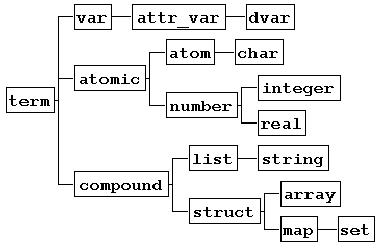
\includegraphics[scale=1]{res/tipi}
	\end{figure}

\end{frame}